\documentclass{ctexart}
\usepackage[utf8]{inputenc}
\usepackage{amsmath}
\usepackage{amsfonts}
\usepackage{mathabx}
\usepackage{tabu}
\usepackage[margin=4cm]{geometry}
\usepackage{pgfplots}
\pgfplotsset{width=10cm,compat=1.9}

\title{人工智能导论 HW3}
\author{计76 刘晓义 2017011426}
\date{2019.6}

\begin{document}

\maketitle

\section{任务复述}
新浪新闻包含一个读者反馈机制:通过在八种情感中选择一种,表示自己看过新闻之后的心情。

本次作业的任务是使用 CNN/RNN 实现对于新浪新闻的情感预测,并作出必要的分析。

总共从三个参数评价模型: 正确率,f-score 以及相关系数。

我使用了 PyTorch 进行实现,代码位于 \url{https://github.com/CircuitCoder/EmotionClassifier},训练得到的模型在 Releases 中。

\section{模型}
\subsection{语料量化}
考虑三种不同的方式:
\paragraph{Bag of Words}
假设词典大小为 $D$, n-gram 中的 Bag of Words 会将语段处理成 $D^n$ 维度的向量,每个维度表示这个 n-gram tuple 在语段中出现的次数。相比于 TF-IDF 无法理解关键词,最后得到的向量中突出的是大量不重要的代词、介词。

\paragraph{TF-IDF}
相比于 Bag of Words, TF-IDF 由于额外考虑了 IDF, 能凸显出更重要的词汇。

存在的问题是在本例中训练数据集比较小,覆盖的单词只能是词典的一小部分,在测试中可能真正能表达文章主旨的词并没有在词典中出现,结果只能使用文章中无法表达主旨,但是出现次数比较少的词汇进行预测,比如地名、人名、时间等等,显然没办法得到正确的情感预测。

\paragraph{Word Embedding}
通过把每个词变成一个固定长度的向量,每个维度代表词在表达这个维度对应意义的程度,所以意思相近的词会在 Word Embedding 之后得到接近的向量。

这种方法的问题和 TF-IDF 类似,都会受到较小训练集的影响。但是可以使用预先训练好的模型,所以即使训练集比较小,也可以在这一步中对词汇得到比较好的理解。

以 CNN 实现为例,在使用预训练的模型之前,CNN 训练收敛后得到的正确率大约 $44\%$,使用预训练的模型后正确率大约 $55\%$

\subsection{CNN}
首先通过对输入进行 Padding,获得长度相等为 L 的一维向量输入。

通过维度 300 的 Word Embedding,得到 $L \times 300$ 的输出。

使用 ${2,3,4} \times 300$ 三种不同大小的卷积核,各 128 个通道的输出,随后大小为 2 的 max pool,得到 $L \times 192$ 的输出。

dropout 之后 full connect,得到长度为 8 的向量,代表每个分类的评分。

之后应该再进行一次 Softmax,得到每个分类的概率。但是在 PyTorch 中,计算交叉熵会隐含一个 Softmax,而在测试集上测试得到正确率只需要找出最大的分量,在这点上 Softmax 是单调的,所以省略这一步也可以。

\subsubsection{参数}

\paragraph{卷积核的大小}
由于不知道 Word Embedding 中每个分量的意义,在这个维度上进行卷积是意义不明的。所以卷积核在这个方向上大小应该和 Word Embedding 的输出维度相等(300),也就是每次卷积操作肯定能考虑到词语的每个意思。

在词的排列维度上,大小为 $n$ 的卷积核能同时考虑到 $n$ 个词汇,得到的效果类似 n-gram。最终选择的三种卷积核分别是 2,3,4。考虑到中文句子组成比较复杂,单独依赖卷积核中单词的相对位置判断在句子中的成分是不太可行的,因此没有选择更大的卷积核。

\paragraph{通道数}
卷积层的通道数也就是抽取出来的特征数。选择每个大小的卷积核各 128 个通道,总共 384 个通道,大约和 Word Embedding 得到的维度一致,希望这一步可以把位置相接近的词之间共同考虑,而不损失什么特征。如果通道数开的太多,Overfitting 的问题会更加严重。

\paragraph{池化函数}
使用了比较常见的 MaxPool,得到在大致位置上某个特征的强度。

猜测可以减少全连接层的大小,一定程度上环节 Overfitting 的问题。

\paragraph{多卷积层}
多卷积层应该是好的,可以得到更大范围的特征,但是由于我真的不会用 PyTorch,只能放弃...

\subsection{RNN}
和 CNN 相同的 Word Embedding 设置。

对不定长的输入进行 Packing / Unpacking 处理。

RNN 使用单向的 LSTM 单元,隐藏特征大小 256,内部 2 层。两层之间有 Dropout。

最终取出最后一个词对应的输出,得到 256 维度的向量,Dropout 之后 Full connect 得到长度为 8 的向量。

\subsubsection{参数设置}
LSTM 确实让训练变快了很多...最后的正确率基本没有区别。

隐藏特征大小 256,层数 2 参考了 \url{https://github.com/keishinkickback/Pytorch-RNN-text-classification} 的默认设置(128, 2),扩大了隐藏特征是因为玄学原因,比 128 稍微好一点。

\section{训练}

\subsection{基本设定}

使用 Adam optimizer, 初始 Learning Rate 0.001, 达到任意以下两个指标停止训练:

\begin{itemize}
\item 600 Epochs
\item 正确率达到 54\%
\end{itemize}

设定两个条件的原因是发现在训练中非常容易出现 Overfitting,即使 Dropout 层的概率设置到 0.8,无论是 CNN 还是 RNN 依旧会在 100 Epochs 左右之后出现正确率下降。经过屡次测试,发现测试正确率最高能达到 55\% 到 57\% 附近,因此选择达到 54\% 的时候就停止训练。


\subsection{训练集、测试集生成}
训练集每次打乱之后切分成 100 个数据一个 Batch,总共测试数据能切分成 22 组,剩下的零头扔掉。22 组训练完成后重新打乱。

由于 PyTorch 的 Packing/Unpacking 实现,这样得到的每个 Batch 还要根据长度降序排列。

测试集直接使用所有测试数据。直接作为一个 Batch 喂给 CUDA 非常容易导致显存爆掉然后 Buy more RAM,所以拆成和训练集一样 100 个数据一组进行测试。

\section{测试结果}

F-Score 的计算使用了 SciKit-Learn 提供的函数: sklearn.metrics.f1\_score,输出得到了 Macro, Micro 和 Weighted 三种不同计算方法的 F-Score

相关系数本身存在一定歧义,我的解读是得到每个数据点的真实分类和 NN 给出的分类,对这两个向量计算 Pearson Correlation。这个使用了 SciPy 提供的函数 scipy.stats.pearsonr

最终的测试结果如下:


\begin{table}[ht]
\centering

\begin{tabular}{|c||c|c||c|c|c|c|c|}
\hline
模型 & Epochs & 训练Acc & Acc & F(Macro) & F(Micro) & F(Weighted) & Cor \\
\hline
\hline
CNN & 240 & 75.00\% & 54.67\% & 0.27241 & 0.54443 & 0.49173 & 0.38097 \\
\hline
RNN & 600 & 71.00\% & 50.00\% & 0.23822 & 0.50000 & 0.44325 & 0.23784 \\
\hline
\end{tabular}
\end{table}

从下图中可以看出,RNN 的测试正确率并没有达到阈值 54\%,在训练后期下降。最高的 Acc 在 240 轮出现,为 53.46\%

\begin{tikzpicture}
\begin{axis}[
    title={CNN},
    xlabel={Epoch},
    ylabel={\%},
    xmin=0, xmax=240,
    ymin=0, ymax=100,
    xtick={0,240},
    ytick={0,20,40,60,80,100},
    legend pos=north west,
    ymajorgrids=true,
    grid style=dashed,
]

\addplot[
    color=red,
    mark=circle,
    ]
    coordinates {
    (10,41.517056)(20,42.549372)(30,44.075404)(40,46.947935)(50,47.666068)(60,50.2693)(70,50.718133)(80,50.628366)(90,51.436266)(100,51.929982)(110,52.648115)(120,52.827648)(130,51.840215)(140,53.366248)(150,52.558348)(160,52.962298)(170,49.86535)(180,53.994614)(190,53.141831)(200,53.411131)(210,53.141831)(220,53.366248)(230,53.904847)(240,54.443447)
    };
 
\addplot[
    color=blue,
    mark=square,
    ]
    coordinates {
    (10,38)(20,45)(30,40)(40,47)(50,46)(60,44)(70,53)(80,45)(90,52)(100,50)(110,45)(120,55)(130,60)(140,52)(150,65)(160,62)(170,59)(180,58)(190,59)(200,67)(210,66)(220,57)(230,71)(240,75)
    };
 
\end{axis}
\end{tikzpicture}

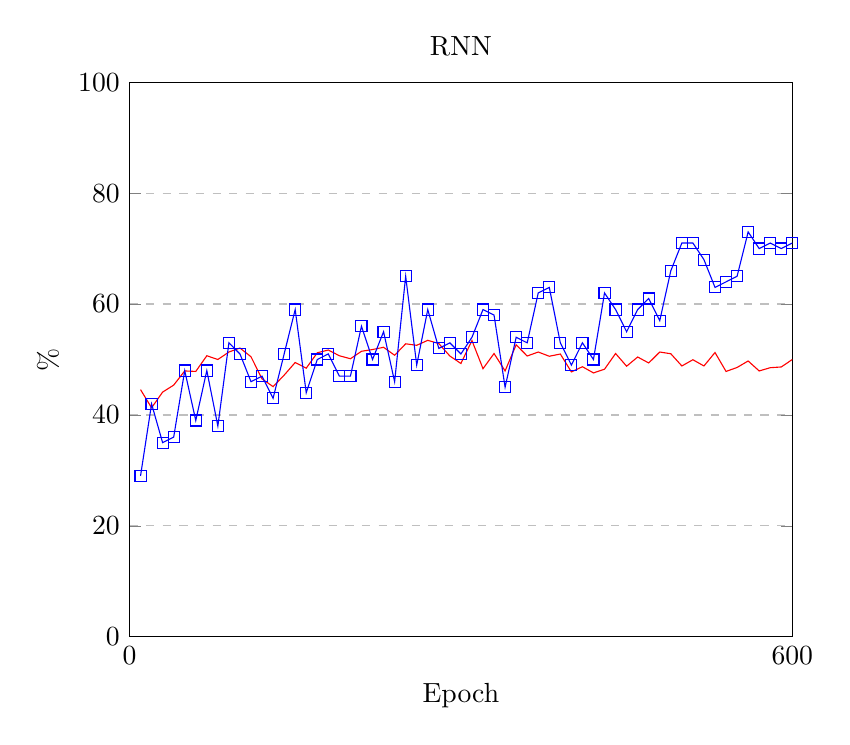
\begin{tikzpicture}
\begin{axis}[
    title={RNN},
    xlabel={Epoch},
    ylabel={\%},
    xmin=0, xmax=600,
    ymin=0, ymax=100,
    xtick={0,600},
    ytick={0,20,40,60,80,100},
    legend pos=north west,
    ymajorgrids=true,
    grid style=dashed,
]

\addplot[
    color=red,
    mark=circle,
    ]
    coordinates {
    (10,44.56912)(20,41.292639)(30,44.120287)(40,45.37702)(50,47.935368)(60,47.845601)(70,50.67325)(80,50)(90,51.346499)(100,52.064632)(110,50.493716)(120,46.499102)(130,45.10772)(140,47.172352)(150,49.4614)(160,48.429084)(170,51.211849)(180,51.705566)(190,50.67325)(200,50.13465)(210,51.481149)(220,51.795332)(230,52.199282)(240,50.763016)(250,52.827648)(260,52.558348)(270,53.456014)(280,52.872531)(290,50.628366)(300,49.281867)(310,53.411131)(320,48.339318)(330,51.077199)(340,47.935368)(350,52.648115)(360,50.628366)(370,51.346499)(380,50.583483)(390,50.987433)(400,47.755835)(410,48.698384)(420,47.576302)(430,48.249551)(440,51.077199)(450,48.788151)(460,50.448833)(470,49.371634)(480,51.346499)(490,51.032316)(500,48.833034)(510,49.955117)(520,48.833034)(530,51.256732)(540,47.845601)(550,48.563734)(560,49.7307)(570,47.935368)(580,48.518851)(590,48.653501)(600,50)
    };
 
\addplot[
    color=blue,
    mark=square,
    ]
    coordinates {
    (10,29)(20,42)(30,35)(40,36)(50,48)(60,39)(70,48)(80,38)(90,53)(100,51)(110,46)(120,47)(130,43)(140,51)(150,59)(160,44)(170,50)(180,51)(190,47)(200,47)(210,56)(220,50)(230,55)(240,46)(250,65)(260,49)(270,59)(280,52)(290,53)(300,51)(310,54)(320,59)(330,58)(340,45)(350,54)(360,53)(370,62)(380,63)(390,53)(400,49)(410,53)(420,50)(430,62)(440,59)(450,55)(460,59)(470,61)(480,57)(490,66)(500,71)(510,71)(520,68)(530,63)(540,64)(550,65)(560,73)(570,70)(580,71)(590,70)(600,71)
    };
 
\end{axis}
\end{tikzpicture}


可以发现正确率都不高...比较显然的一个问题是 Overfitting。虽然尝试使用了一些办法解决(具体见问题思考),但是没有成功。

\section{问题思考}

\subsection{终止条件}
如训练一节所叙述,固定代数容易因为代数太多而 Overfit。优点是很稳定,保证能够收敛到一定的范围内。

如果只依赖正确率,优点是没有上面的问题,但是如果正确率没有达到预计结果,那么继续训练会导致 Overfitting 越来越严重。同时,如果在训练初期,一个接近随机的权值对选中的测试数据恰好效果很好,那么这时候终止训练可能导致在真实应用中对更多数据的效果不好。

\subsection{权值初始化}

PyTorch 默认是根据不同的权值选择不同的初始化方法。对于实现中所使用的大多数(Conv, LSTM),都是使用在 0 附近的正态分布作为初始化。

使用 0 初始化可以保证模型一开始得到的结果不会飘得太远,这样可能离全局最小值更近。但是全都用 0 的话也更可能会遇到正好陷进局部最小值,或者遇到梯度很小的情况,这时候训练就进行不下去了,所以可以使用正态分布或者正交初始化。

\subsection{防止过拟合}
在我的实现中主要通过添加 Dropout 以及减小 Full connect 层的大小。

其中,添加 Dropout 的效果最为明显。虽然会稍微降低训练速度。大约提升了 5\% 的正确率

除此之外,减小 Full connect 层提升了 3\% 的正确率。

减小网络大小也可以一定程度上防止过拟合,但是网络的正确率下降的太多,所以得不偿失。

\sbusection{RNN,CNN 相比于全联接的优势}

猜测 RNN,CNN 和全联接网络的区别主要在于复用了同一个结构以及其中的权值,应用在了输入的多个部分上。

这样第一减小了训练的时间,并且在语义上也是说的通的:我在输入的前半段找特征 A,和我在后半段应用的方法应该差不多才对。  这样对特征出现在输入中的位置没有全联接层那么敏感,所以能够减小 Overfitting 的可能性。 
\end{document}

